%% Outline
% 1. Navigation is important problem
% 1.5 Traditionally addressed by mapping during exploration and path
%      planning during exploitation.
% 2. End to end learning algorithms have shown promise to take over
%      mapping and path
% 3. We do not know how these algorithms work. There has been work in computer vision that shows the learning on neural network based methods can be learning totally different kind of patterns from what we would expect.
% 4.1 We find that it is not remembering the map it is being trained on
% 4.2 We find that no path planning is  happening only, memorizing and regeneration of the sequence of steps. However, it is not 

% 1. Navigation is important problem
% 1.5 Traditionally addressed by mapping during exploration and path
%      planning during exploitation.
Navigation remains a fundamental problem in mobile robotics and artificial intelligence~\cite{SmChIJRR1986,ElCOMPUTER1980}.
The problem is classically addressed by separating the eventual task of navigation into exploration and exploitation. 
In exploration the environment is represented in some sort of \emph{map} data-structure. 
In exploitation, the map is used for localization and path-planning to find a path to a desired destination based on given optimality criterion. 
This classical approach, traditionally called SLAM (Simulataneous Localization and Mapping), constitutes an entire subfield of robotics whose successes include the birthing of the autonomous driving industry. 
SLAM however, possesses its own limitations. Algorithms, especially those centered in vision, lack performance invariance often failing to extend results to environments that are subtly different from the ones they were trained on. As a simple example, state-of-the-art monucular SLAM methods fail when confronted with textureless environments.

More recently, end-to-end navigation methods---methods that attempt to  
solve the navigation problem without breaking it down into separate parts of localization, mapping and path-planning---have gained traction.
%
% 2. End to end learning algorithms have shown promise to take over
%      mapping and path-planning
With the recent advances of Deep Reinforcement Learning (DRL) \cite{MnKaSiNATURE2015}, these end-to-end navigation methods \cite{MnBaMiICML2016,SiHuMaNATURE2016,LePaKrISER2017,MiPaViICLR2017,OhChSiICML2016} forego decisions about the details that are required in the intermediate step of mapping.
The potential for simpler yet capable methods is rich; for example, agents thus trained would be expected to optimize to store only the minimal amount of map information that is required to perform the end objective of a navigation task.
One such work, \cite{MiPaViICLR2017}, has demonstrated algorithms that are able to explore and find goals in complicated three-dimensional worlds utilizing only the monocular front-facing view of these agents. Of signficance is the fact these agents upon finding the goal within a previously seen environment, are able to navigate to it faster in subsquent explorations implying that agents are able to learn to exploit map structures in the execution of learned navigational tasks. 

\begin{figure}
%\rotatebox{90}{\hspace{3em}Trained on 1 map }
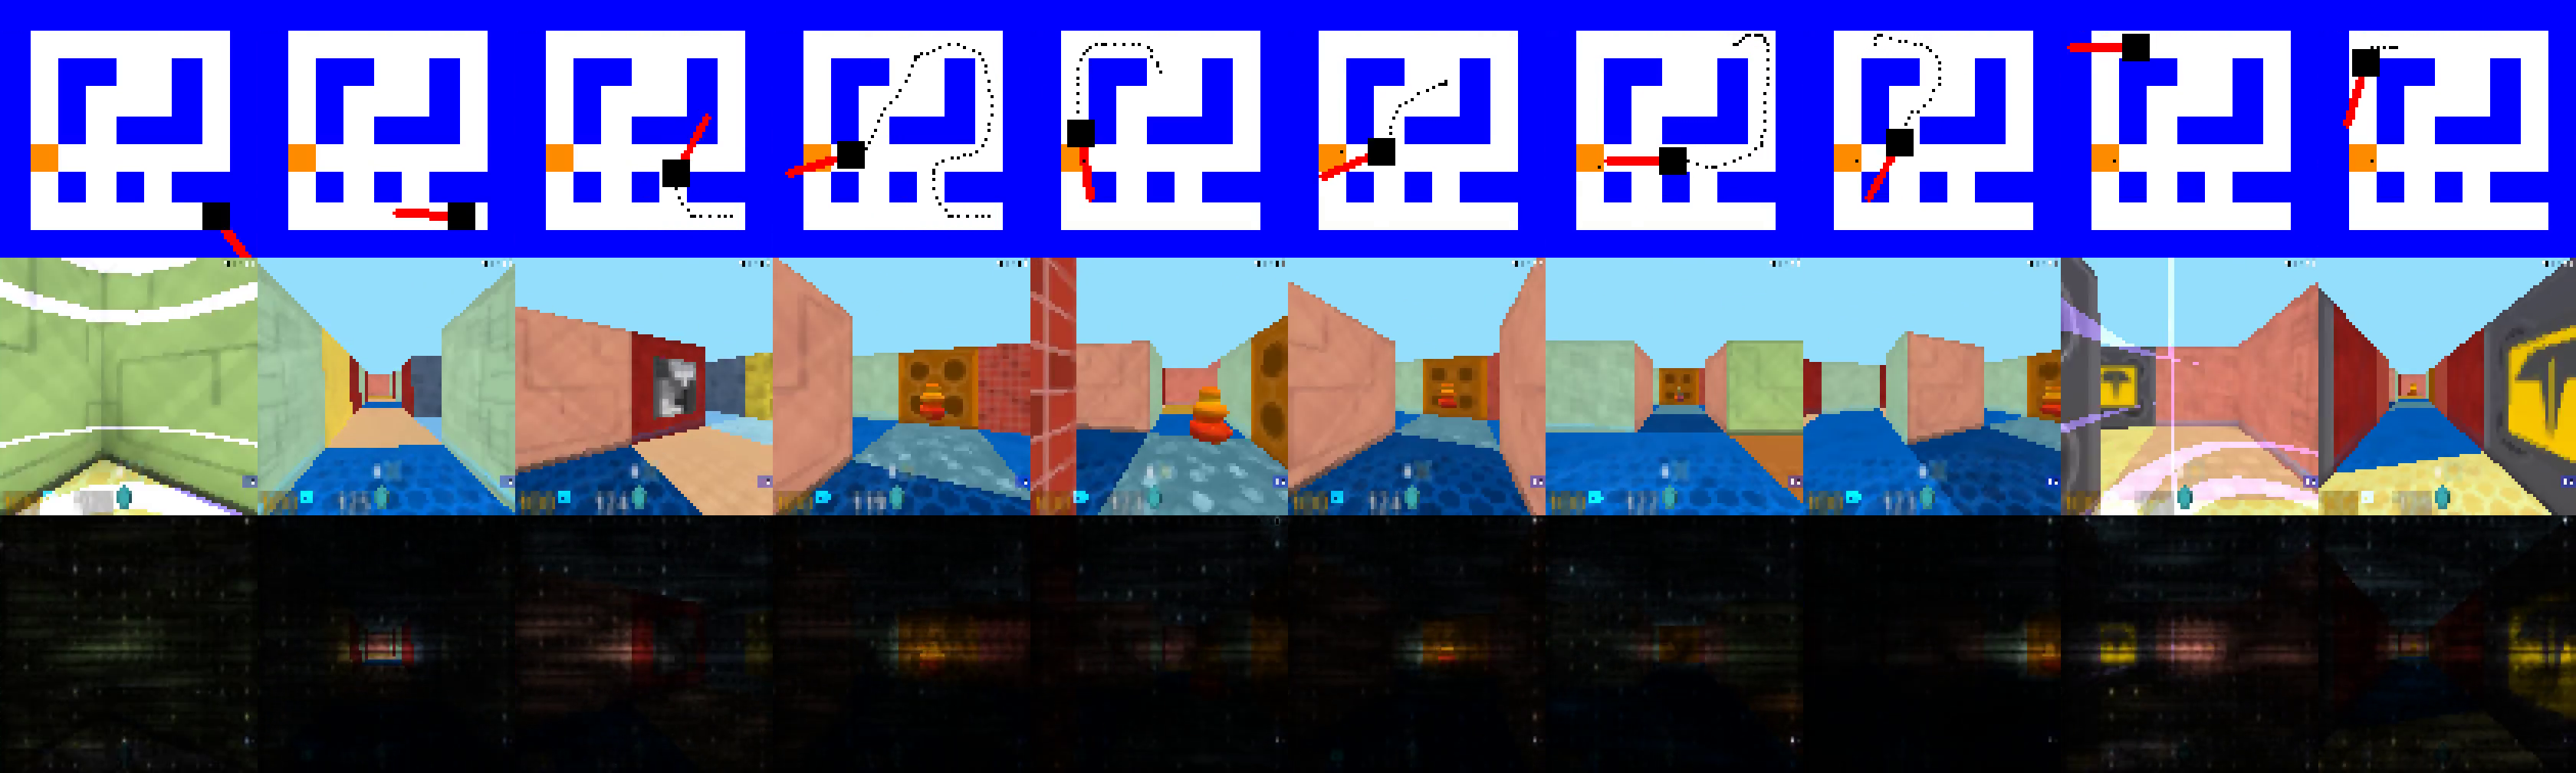
\includegraphics[width=\textwidth]{./exp-results/training-09x09-0127-on-0127.png}%
%\rotatebox{90}{\hspace{2em}Trained on 1000 maps }
%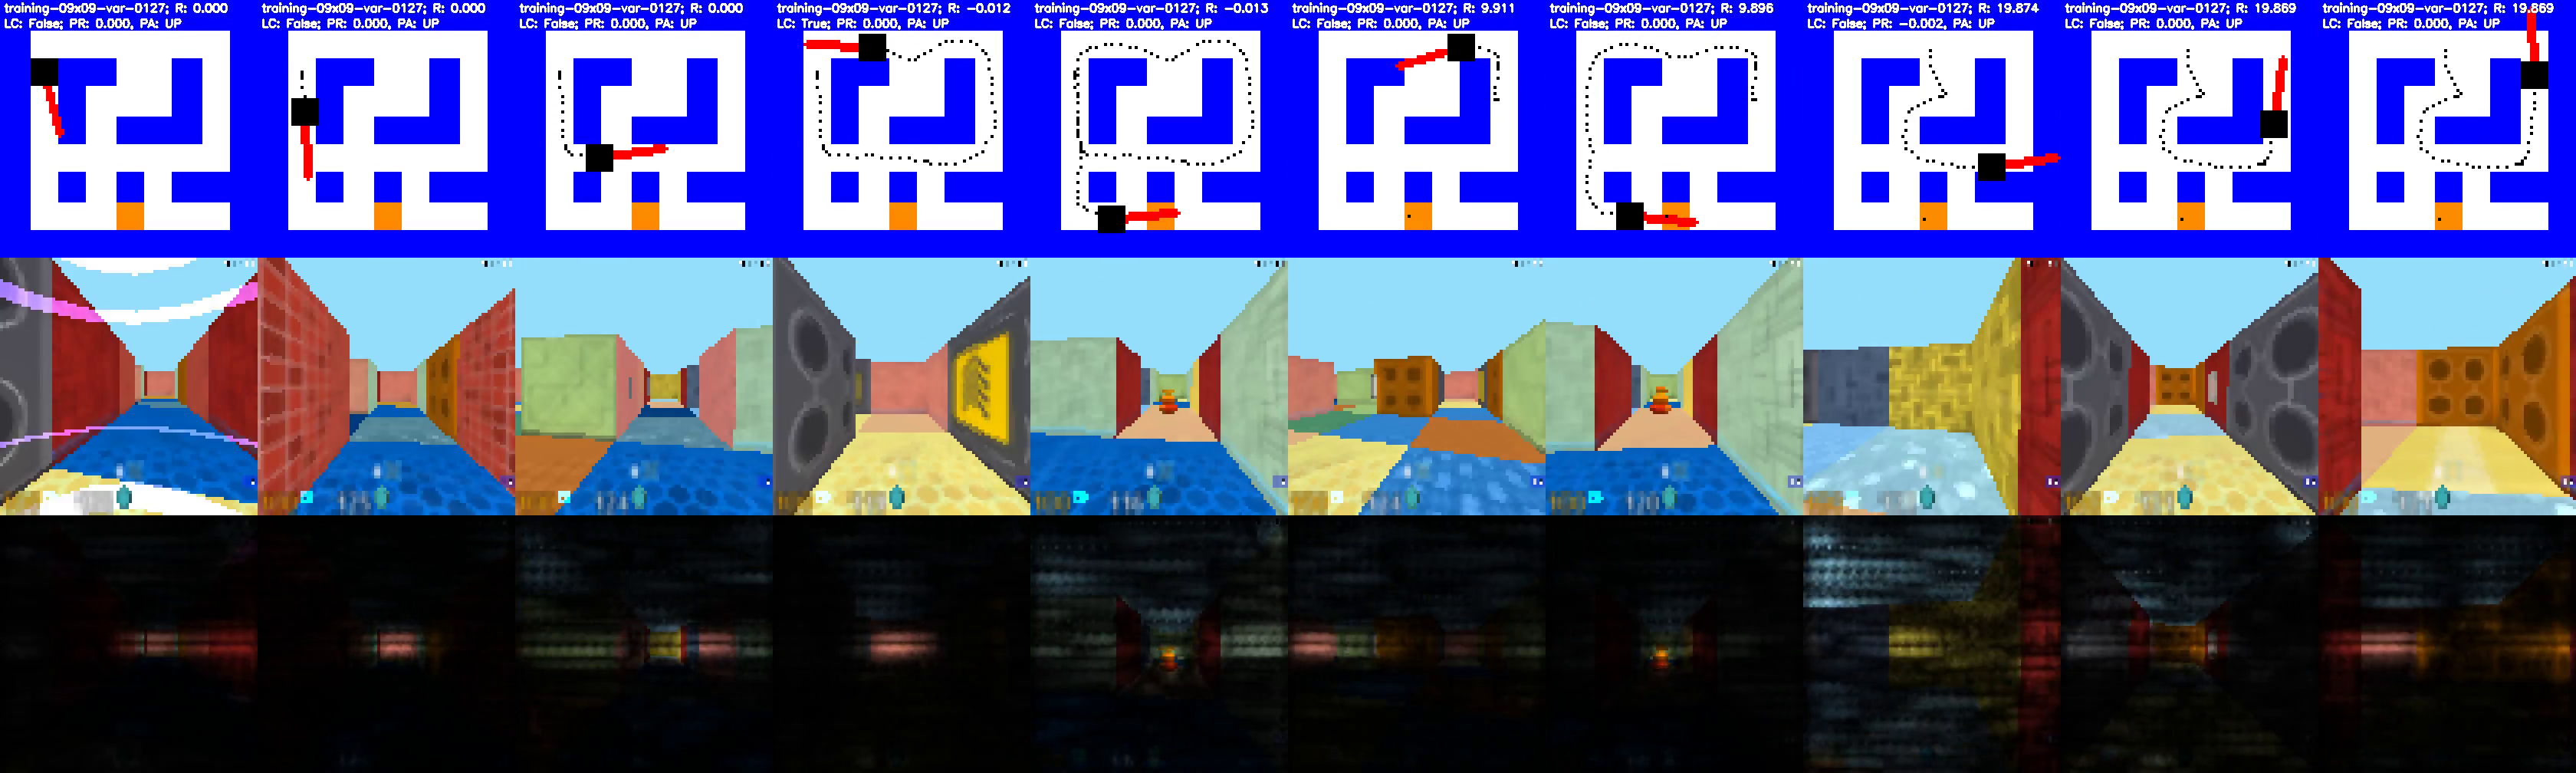
\includegraphics[width=\textwidth]{./exp-results/training-1000-on-0127.png}
\caption{Qualitative results of evaluating algorithm on map id 127. The top three rows show selected frames for the algorithm trained on the same map 127, while the bottom three rows show the result of evaluting the algorithm trained on 1000 maps evaluated on 127. The top row shows the top view of the robot moving through the maze, second row shows the first person which is the only input available to the agent (except reward). The third row shows the attention masked view of the algorithm. We observe that the algorithm focuses attention at the horizon in long corridors, on the goal object (it looks like stacked rings) and on interesting decals.}
\label{fig:training-qualitative}
\end{figure}

% 3. We do not know how these algorithms work. There has been work in computer vision that shows the learning on neural network based methods can be learning totally different kind of patterns from what we would expect.
Despite such potential advances, DRL based navigation remains a relatively unexplored field with its own set of limitations. 
The black-box nature of these methods make them hard to study and the underlying patterns captured by the agents are not understood. 
Their exists no comprehensive set of experiments that answer how and when these algorithms perform well and how their performance differs based on variations in the training and testing conditions. 
It is also unknown whether such algorithms are able to extend learned abilities to previously unseen worlds to complete the navigation task.
With earlier work such as \cite{NgYoClCVPR2015} already establishing that  neural-network-based object detection methods can be easily fooled by introducing noise that is imperceptible to humans, it is important to analyze these DRL methods across a wide variety of experiments to understand the extent of their navigational abilities \cite{MiPaViICLR2017}.

% 4.1 We find that it is not remembering the map it is being trained on
% 4.2 We find that no path planning is  happening only, memorizing and regeneration of the sequence of steps. However, it is not 

In this work, we build of the efforts of \cite{MiPaViICLR2017} and analyze their methods across hundreds of maps with differing degrees of randomness. 
Our setup is similar to theirs utilizing the same open-source library, Deepmind Lab \cite{BeLeTeARXIV2016}, for experimentation. i
We randomly genereate our mazes wherein the agent and goal are both statically and randomly spawned across experiments. 
Agents are tasked to learn to navigate the environments to maximize reward over episodes of fixed time lengths.

In the case where the goal is randomly initialized within environments that have been previously been trained on, \cite{MiPaViICLR2017} showcase that their agents are able to exploit map structures to maximize reward. However, their experiments are not comprehensive enough to rule out random chance as they show this successful result on only one map while not reporting the standard deviations across their metrics. It is also unclear whether this observed exploitation extends to previously unseen environments as their agents are trained and tested on the same maps. Even though separating training and testing sets is standard practice in machine learning, to the best of our knowledge, we are the first work to evaluate any DRL based navigation method on unseen maps. 

To address this lacks of information about these agent's navigational abilities, we systematically expand upon \cite{MiPaViICLR2017}'s analysis by evaluate these agents and  metrics on a comprehensive set of randomly generated maps with differing training and testing conditions of increasing complexity. 
In particular, we move from deterministic setups wherein the agents are trained on environments containing fixed spawn points, fixed goal locations and coincident training/testing maps to  much more complex cases involving random spawn points, random goal locations and diverged training and testing sets. 
In particular, we quantitavely evaluate our trained models to test their map-exploitation abilitiesacross these differing setups and observe agents are unable to transfer this ability to the unseen worlds. Instead we observe that the agent's preferred path to the goal is just as an artifact of its initialized location and rotation and hypothesize that the agents are learning a correspondence between local sequences of frames and actions that lead to the goal.

We also compute attention-maps for these agents in a bid to understand the kind of features used in the context of their navigation. We find that the agents discard most of the information provided to them instead focusing attention on a small band in the middle of the monocular view provided to them. We provide qualitative results and quantitative numbers backing up this claim.

These findings are the results on training and testing on multiple maps that were randomly chosen from a set of 1100 randomly generated maps. We provide thorough and clear summaries of our data to substantiate these findings as well as individual maps and results to explain them carefully. Our findings are available and reproducible at this github link.
